\byline{{\textbf{\Large\sffamily Bonsai Almanac:}}\\
        {\textbf{\large\sffamily A Monographic Guide to Pines}}}{Stefano Bragaglia}
\label{2025-11-almanac}
\vspace*{-1em}
\noindent
The pine bonsai represents one of the most fascinating and complex disciplines within the art of bonsai.
Each species possesses a unique vegetative behaviour, its own sensitivity to environmental changes and a characteristic response to traditional cultivation techniques.
The information contained in this article derives from the reworking of the material presented by Diego Fortuna, bonsai instructor with over 25 years of experience and founder of the \href{htthttps://www.fortunabonsaischool.it}{Fortuna Bonsai School}, during two highly detailed conferences in which he shared the experience gained over more than twenty\--five years of cultivation, refined thanks also to his studies in Japan with Master Urushibata of Taisho\--en.

The aim is to offer a structured and complete guide that accompanies the reader from understanding the various pine species to the fundamental techniques, right through to the management of the plant's entire annual cycle, month by month.
At the end, a section dedicated to the development of pines in the pre\--bonsai stage is also included, for those still far from fine maintenance and who need to build structure and vigour.

\medskip
\topic{\large\sffamily Pine varieties in bonsai:\\ characteristics and differences}
\label{varieta}
\noindent
In the bonsai world, the most commonly used pine species include the Japanese black pine (\textit{Pinus thunbergii}), the Japanese white pine (\textit{Pinus parviflora}), the Japanese red pine (\textit{Pinus densiflora}), the Scots pine (\textit{Pinus sylvestris}), the mountain pine (\textit{Pinus mugo}), the eastern white pine (\textit{Pinus strobus}) and, although not a pine, also the Japanese larch (\textit{Larix kaempferi}, known as karamatsu), often considered within the same techniques due to seasonal and physiological analogy.

\begin{window}[2,l,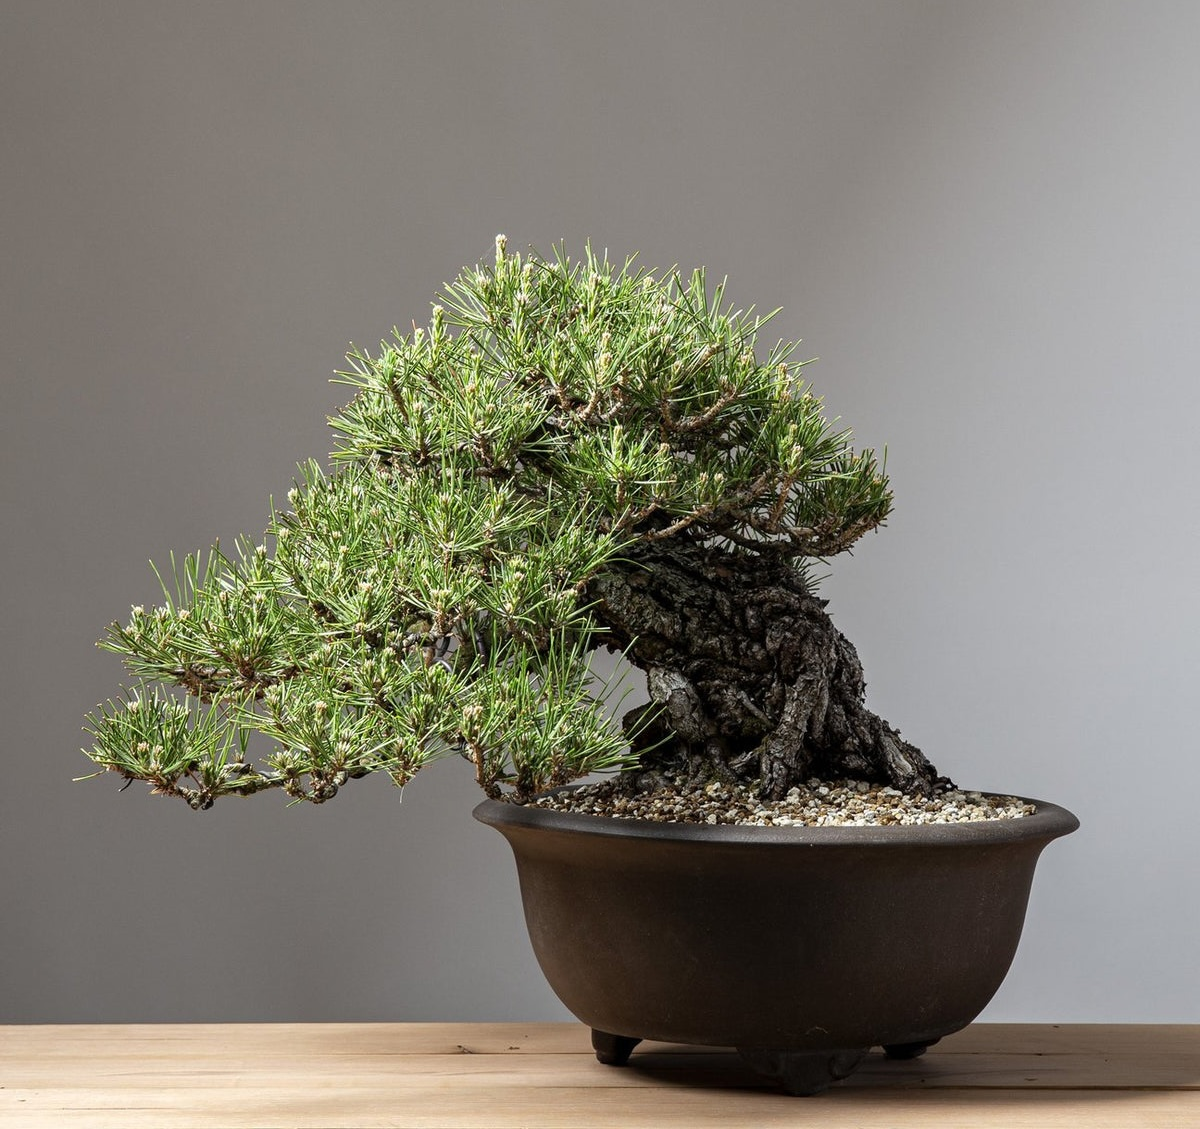
\includegraphics[width=1.0\columnwidth]{2025_11/res/pines_black.jpg},\centerline{\emph{A Japanese black pine (pinus thumbergii).}}]
\end{window}
\columnbreak

All these conifers share several common characteristics: they produce spring candles, form future buds during summer, respond well to organic fertilisers, prefer free\--draining substrates and dislike both summer overheating and severe frosts that directly affect the root ball.
However, each species displays important differences in vigour, needle length, reaction times and sensitivity to interventions.

\begin{itemize}
    \item The Japanese black pine is probably the most vigorous species among those commonly cultivated.
    It has long, stiff needles and shows an exceptional response to \textit{mekiri}, the summer cutting of the candles that induces a second, more compact flush.
    It requires abundant fertilisation, loves heat and tolerates intense sun exposure well, although it is sensitive to pot overheating.

    \item The Japanese white pine, on the other hand, has short and soft needles, more limited vigour and greater overall sensitivity.
    It does not respond in the same way as the black pine to mekiri and requires more delicate interventions.
    It is particularly sensitive to root rot and to excess fertiliser, especially during the warmer months of the year.

    \item The red pine represents an intermediate option: more vigorous than the white, less than the black; it tolerates some techniques derived from thunbergii, while still requiring a more measured approach.

    \item The Scots pine, very common in Europe, adapts well to our climates and responds consistently to spring pinching and bud selection.
It is a tree largely managed through light: well\--lit branches tend to be more vigorous, which allows balanced control of vigour.

    \item The mountain or mugo pine is a montane species that requires\hfill cooler\hfill conditions\hfill and\hfill consistent\hfill moisture.\hfill
\end{itemize}    

\begin{window}[2,l,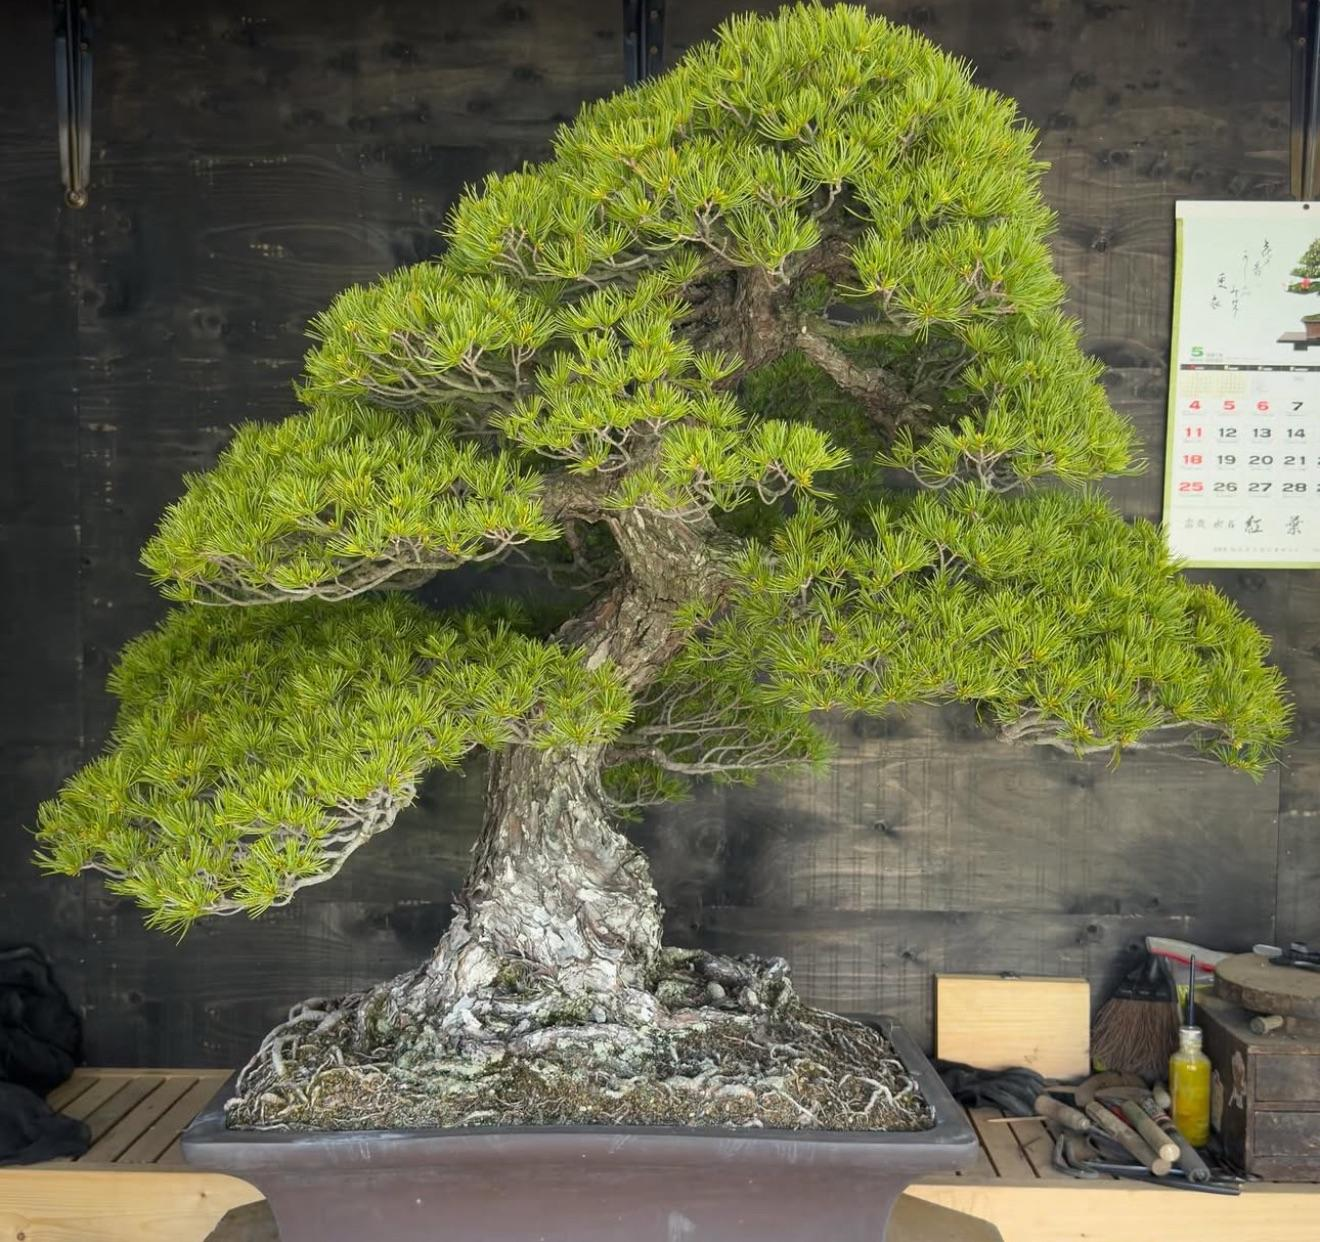
\includegraphics[width=1.0\columnwidth]{2025_11/res/pines_white.jpg},\centerline{\emph{A Japanese white pine (pinus parviflora).}}]
\end{window}
\columnbreak

\vspace*{-3em}
\begin{window}[2,l,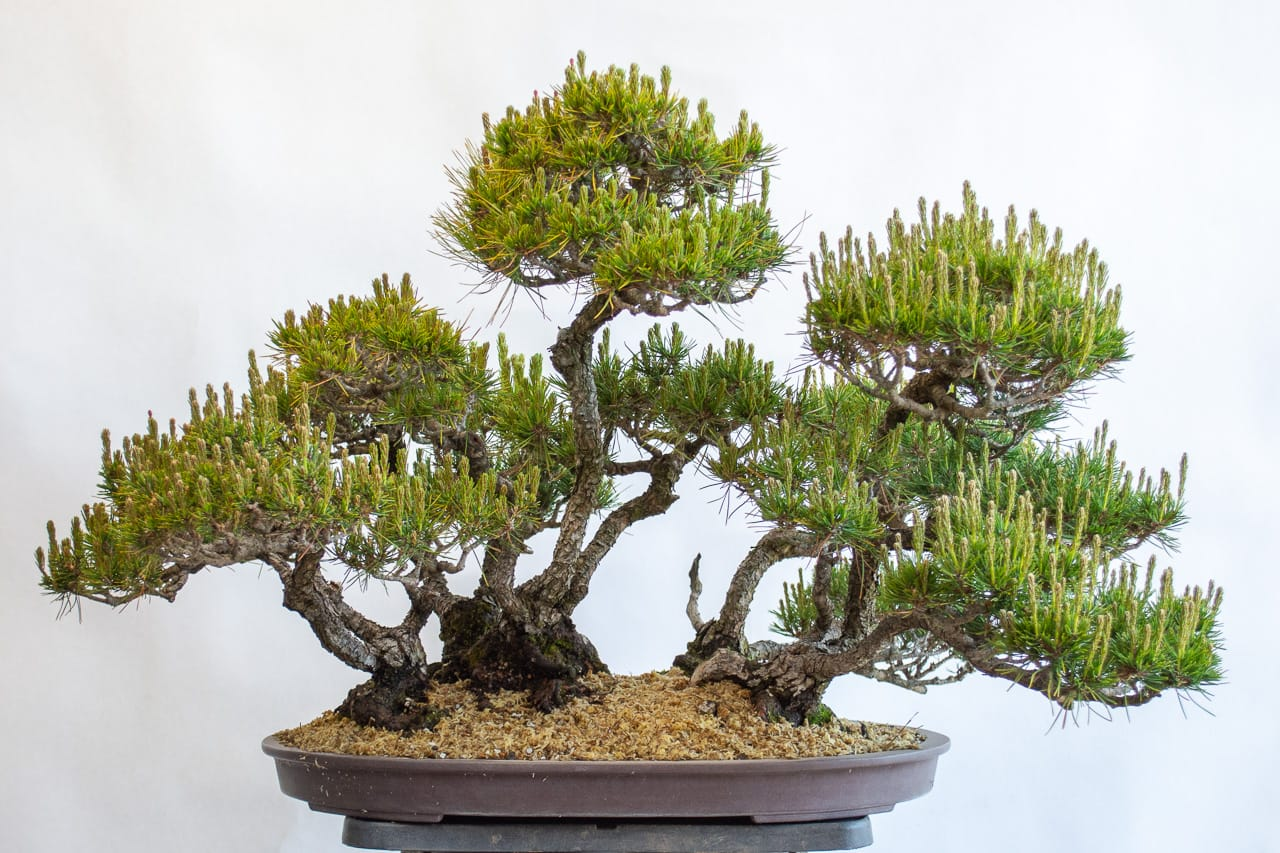
\includegraphics[width=1.0\columnwidth]{2025_11/res/pines_red.jpg},\centerline{\emph{A Japanese red pine (pinus densiflora).}}]
\end{window}

\begin{itemize}
    \item[] It does not tolerate waterlogging, but neither does it cope well with prolonged drought.
    It is sensitive to poorly timed work and is often the subject of mistakes caused by the incorrect belief that it can be managed like the black pine, which is not advisable.

    \item The eastern white pine has very soft and long needles and requires abundant light but fears intense heat and drought, behaving similarly to white pines.

    \item Finally, the Japanese larch, though not a pine, is often treated in parallel due to its seasonal management.
    It is a deciduous conifer that responds very well to pinching and bud selection and prefers cool, bright and humid environments.
\end{itemize}

\medskip
\topic{\large\sffamily Glossary of techniques and Japanese terms}
\label{glossario}
\noindent
To correctly understand and apply bonsai techniques, it is essential to become familiar with some Japanese terms that identify specific operations.
\textit{Mekiri} is the complete cutting of the summer candle when it has finished its primary elongation but has not yet hardened.
This technique, central for black pine, stimulates the production of smaller new buds and improves fine ramification.
\textit{Metsumi}, instead, is the pinching of the candles while they are still soft, before they elongate excessively; it serves to control internode length, balance vigour and maintain the harmonious shape of the tree.

By ``candle'' we mean the new spring growth of the pine, which develops as an elongated cylinder before the needles open, while the ``bud'' is the small cone that forms during summer and will become the following year's candle.
The term \textit{kasane} refers to the selection of buds aimed at eliminating excess ones, maintaining correct growth direction and preventing the formation of multiple whorls.
\textit{Nebari} indicates the base of the trunk and the arrangement of surface roots, while \textit{jinen} identifies a more natural cultivation style, often applied to white pines, which involves fewer forcings and gentler interventions.
\columnbreak

% \medskip
\topic{\large\sffamily Annual cycle of the pine bonsai}
\label{ciclo_annuale}
\noindent
To truly understand a pine bonsai, one must know its annual cycle in depth.
Pines modify their physiological behaviour every month, and each phase corresponds to specific interventions.
What is done (or not done) in a given period directly affects the plant's response in the following months.
Below is a complete overview, from the winter dormancy to the full summer vegetative activity, concluding with the autumn maturation of the buds.

\smallskip
\topic{\sffamily January: the heart of winter}
\noindent
In January the pine is in complete dormancy.
The buds are closed and asleep, the roots work at a minimum, and the plant is unable to react to drastic interventions.
At this time, no structural or maintenance work on the foliage should be carried out.
Protecting the pot from frost is particularly important, especially for more sensitive species such as the white pine, using raisers or insulating materials that prevent the root ball from freezing.
It is a good moment to check for any pests hiding in the crevices of the bark.

\smallskip
\topic{\sffamily February: the pre\--awakening}
\noindent
In February the plant is still dormant but is approaching the root\--awakening\hfill phase.\hfill
Towards\hfill the\hfill end\hfill of\hfill the\hfill month,\hfill under

\vfill

% \vspace*{-3em}
\begin{window}[2,l,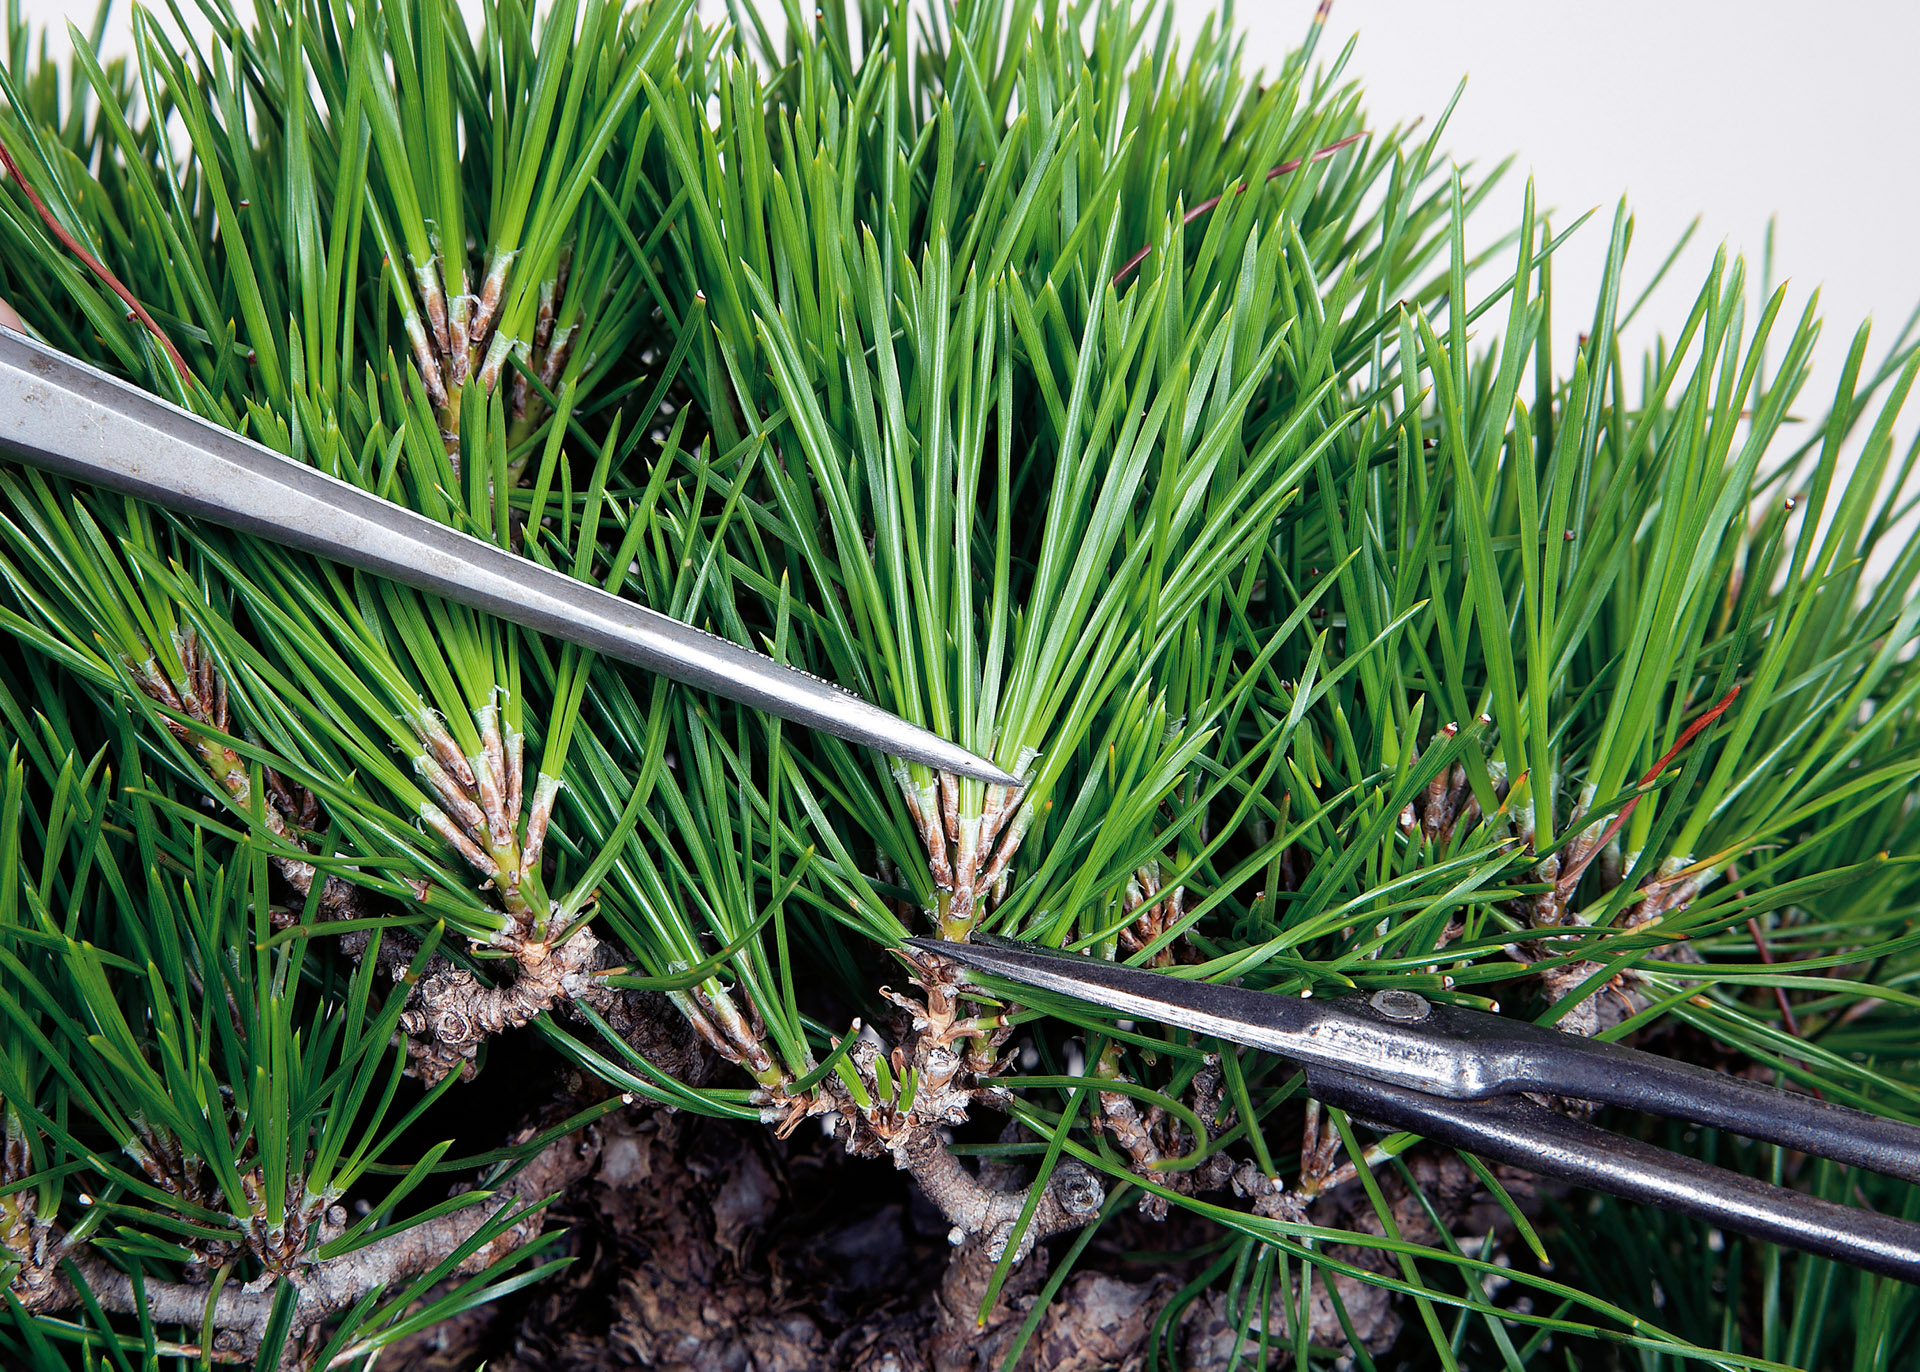
\includegraphics[width=1.0\columnwidth]{2025_11/res/pines_mekiri.jpeg},\centerline{\emph{Mekiri, or complete cutting of the summer candles.}}]
\end{window}

\vspace*{-2em}
\begin{window}[2,l,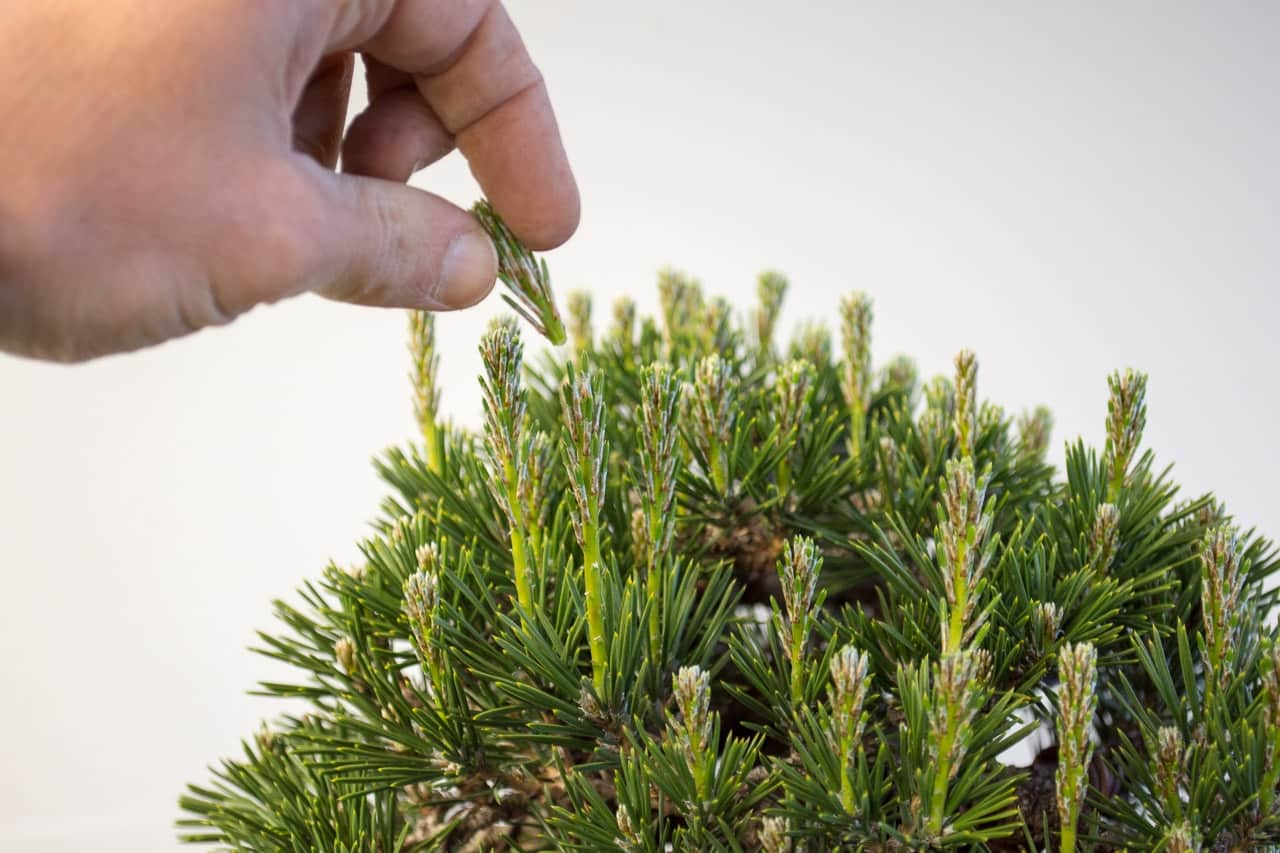
\includegraphics[width=1.0\columnwidth]{2025_11/res/pines_metsumi.jpg},\centerline{\emph{Metsumi, or pinching of soft growing candles.}}]
\end{window}
\columnbreak

\noindent
favourable climatic conditions, repotting can be planned for many species, particularly black and red pines, as well as Scots pines.
Mountain pines require more caution and it is often preferable to wait until March, while white pines should be repotted only if truly necessary, as they are highly sensitive to root stress.
In this month, some light structural pruning can also be carried out, more suitable for black and red pines than for whites.

\medskip
\topic{\sffamily March: the month of repotting}
\noindent
March is one of the most delicate months in the management of pine bonsai.
Root activity resumes, making this period ideal for repotting, always performed before the candles begin to extend.
It is essential to choose an appropriate grain size: coarser for development, finer for maintenance.
Substrates must be free\--draining and airy; a mix of akadama, pumice and kiryu is particularly effective, while parviflora require a higher percentage of akadama.
After repotting, it is important to protect the surface with sphagnum to improve moisture management.
Fertilisation is not yet applied this month: the pine needs to stabilise before being fed.

\medskip
\topic{\sffamily April: the candle\--elongation phase}
\noindent
In April the candles begin to elongate.
It is a crucial moment: the new growth is soft and full of energy.
In this month the candles of Scots pines and mountain pines can be shortened through \textit{metsumi}, pinching their tips to modulate internode length.
In black pines, however, the candles must not be touched: their management will take place later.
Around mid\-- or late April, organic fertilisation can begin, avoiding starting too early so as not to deform the candles.

% \vspace*{-2em}
\begin{window}[2,l,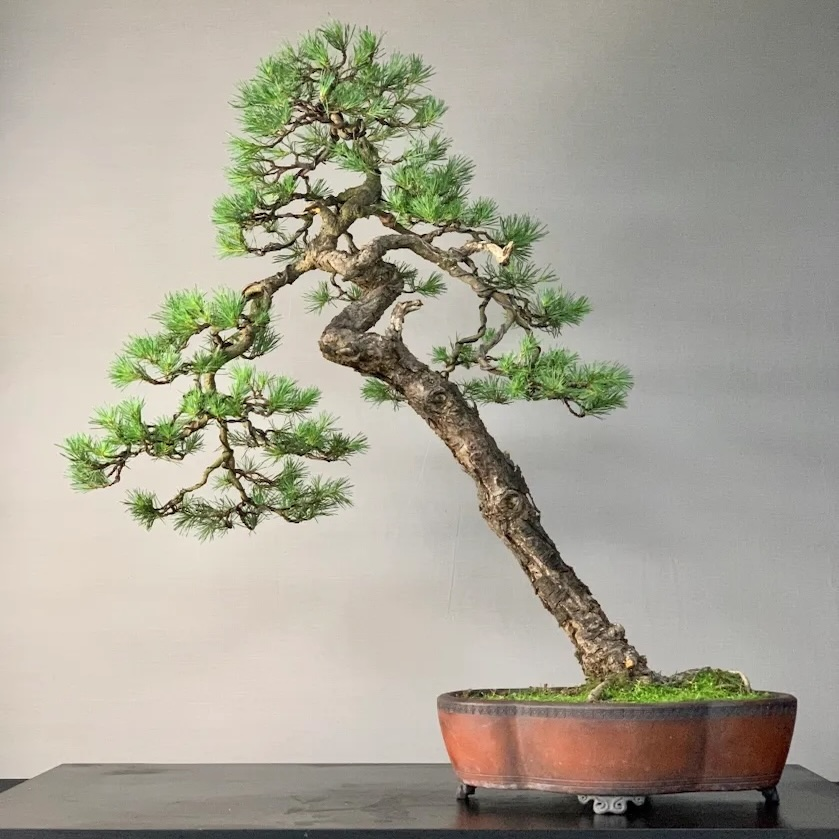
\includegraphics[width=1.0\columnwidth]{2025_11/res/pines_scots.jpg},\centerline{\emph{A Scots pine (pinus sylvestris).}}]
\end{window}
\columnbreak

\medskip
\topic{\sffamily May: candle hardening}
\noindent
May is the month in which the candles begin to harden.
Irrigation\hfill and\hfill fertilisation\hfill must\hfill be\hfill dosed\hfill with\hfill particular\hfill care.

% \columnbreak

\noindent
For mountain pines, this month is important for understanding how the plant is distributing its vigour and correcting any imbalance between the candles.
In Scots pines, light pinching can still be carried out during the first weeks of the month.

\medskip
\topic{\sffamily June: the month of mekiri for black pines}
\noindent
June is the most technical month for the Japanese black pine.
In thunbergii, and in some cases in red pine, \textit{mekiri} is carried out, that is, the complete cutting of the candles.
This technique induces the appearance of new buds and allows short internodes and finer ramification.
Before mekiri, fertilisation should be stopped for about ten days; fertilisation is resumed roughly ten days after the intervention.
White, mountain and Scots pines must not undergo mekiri, as they would react negatively.

\medskip
\topic{\sffamily July: summer re\--budding}
\noindent
In July, black pines produce the new post\--mekiri buds, small and very valuable for the future structure of the plant.
It is essential to protect the trees from excessive heat and direct exposure during the hottest hours.
Moderate fertilisation continues, avoiding excesses that could stress the newly formed buds.
In white pines, this month requires particular attention to hydration management.

\begin{window}[2,l,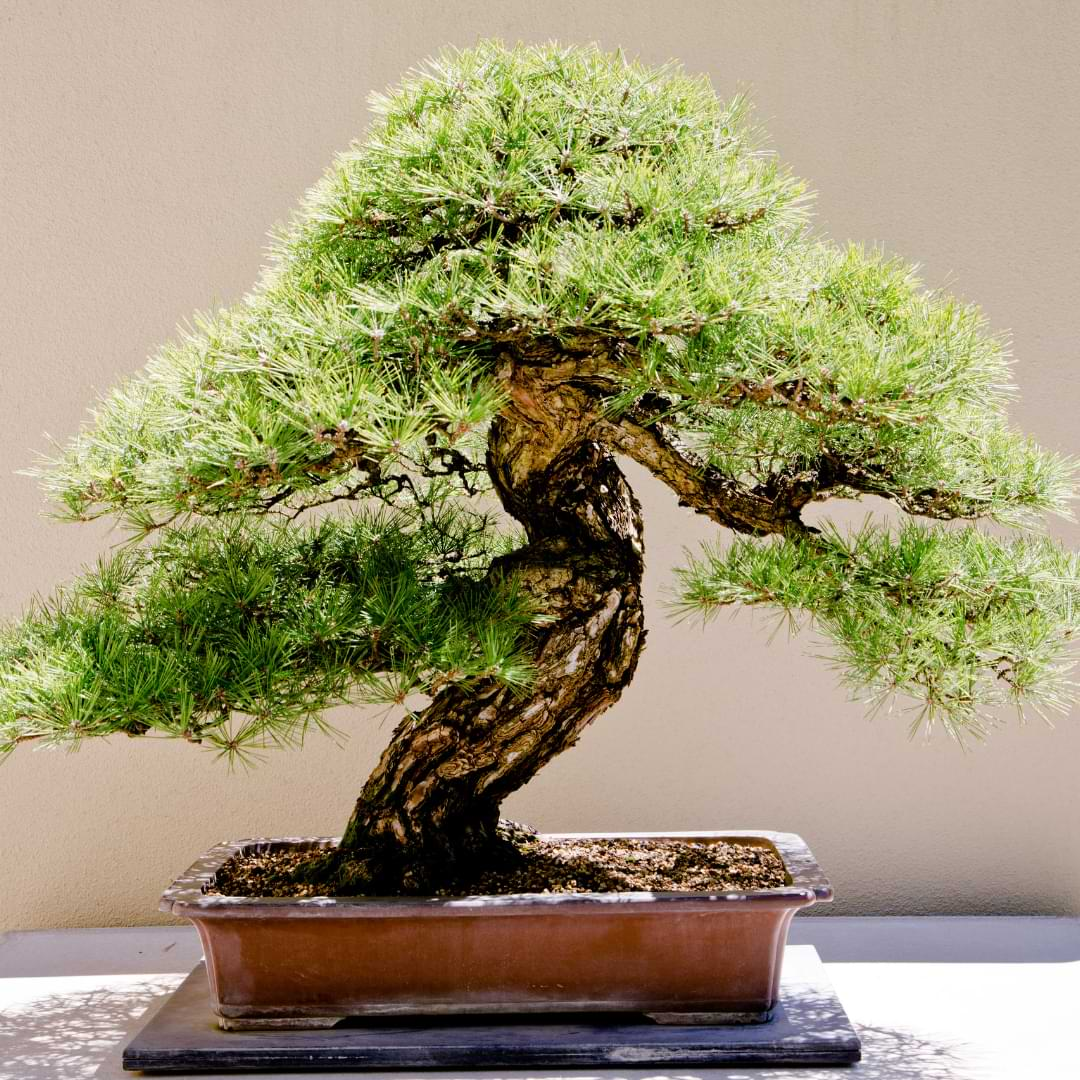
\includegraphics[width=1.0\columnwidth]{2025_11/res/pines_mugo.jpg},\centerline{\emph{A Mountain pine (pinus mugo).}}]
\end{window}
\columnbreak

\begin{window}[2,l,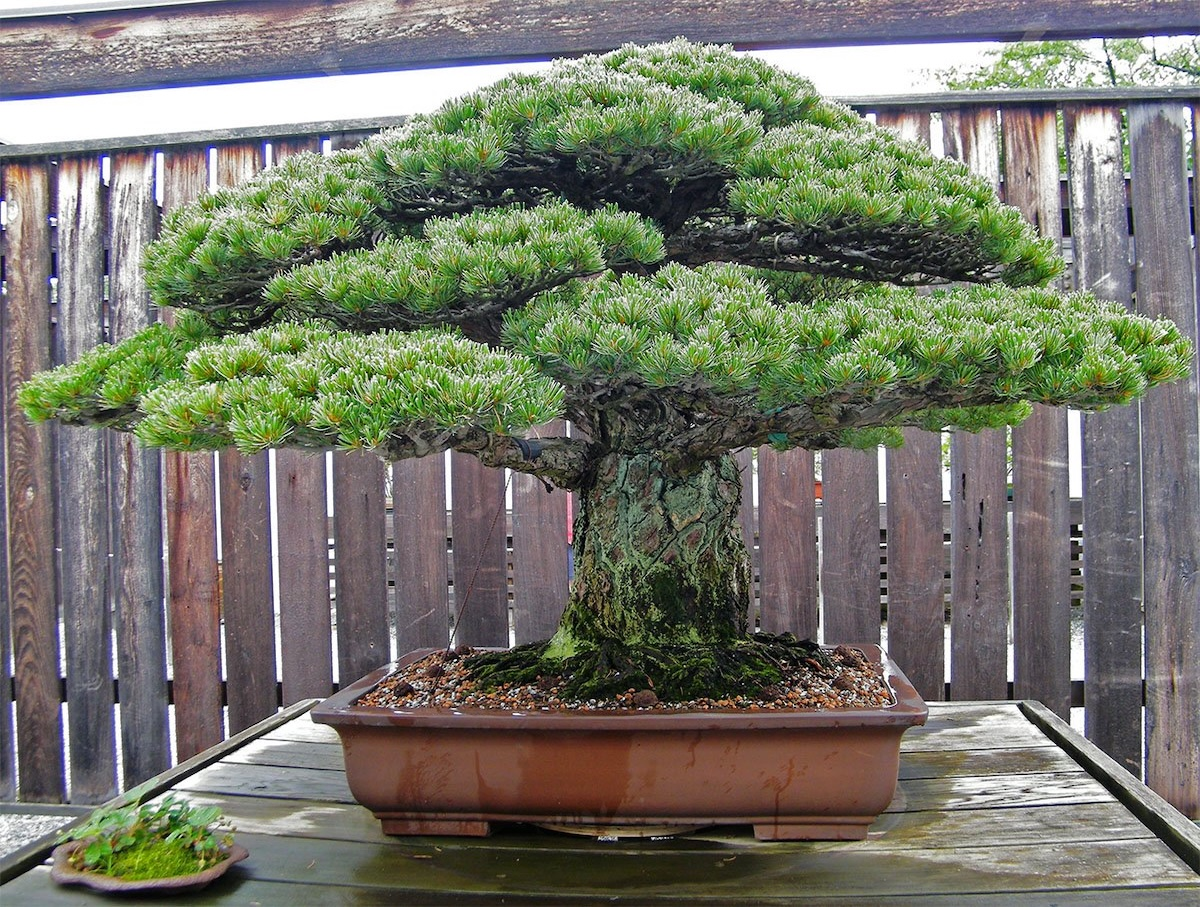
\includegraphics[width=1.0\columnwidth]{2025_11/res/pines_strobus.jpg},\centerline{\emph{A Eastern white pine (pinus strobus).}}]
\end{window}

\vfill 

% \medskip
\topic{\sffamily August: setting the buds for the following year}
\noindent
August is a key transition for all pine species because it is when the plant sets the buds that will produce the following spring's growth.
During this phase, budding is carefully observed to assess quantity, quality and position.
It is the ideal moment to perform \textit{kasane}, the selection of buds, removing the excess and leaving only those most useful for building structure.
For white pines, this phase is critical: excess fertiliser could damage the plant, so it is essential to suspend or reduce feeding.

\medskip
\topic{\sffamily September: bud maturation}
\noindent
September marks the phase of bud maturation and needle hardening.
It is a month dedicated to preparing the plant for autumn and winter.
Fertilisation may resume to encourage the accumulation of reserves that will be useful the following spring.
Old needles on established trees should be removed to allow light and air to enter the canopy.
For white pines, September is one of the most important months of the year, because bud structure will determine the final form of future growth.

\medskip
\topic{\sffamily October: full autumn}
\noindent
October is an ideal month for cleaning old needles and for the final selection of buds.
Cooler temperatures allow light wiring without risking bark damage.
It is also a good month for deadwood work.
Autumn fertilisation continues, preferably with richer organic fertilisers useful for consolidating energy reserves.

\medskip
\topic{\sffamily November: entering dormancy}
\noindent
In November the plants drastically reduce their activity.
The last wirings can be checked, but major work is not advisable.
Fertilisation is stopped and preparations are made for frost protection in the coming months.

\medskip
\topic{\sffamily December: complete dormancy}
\noindent
December is a month of total quiescence.
No biological work is possible.
It is, however, a good moment to evaluate the overall structure of the plant, observe branch arrangement and plan interventions for the following year.

\columnbreak

\begin{window}[2,l,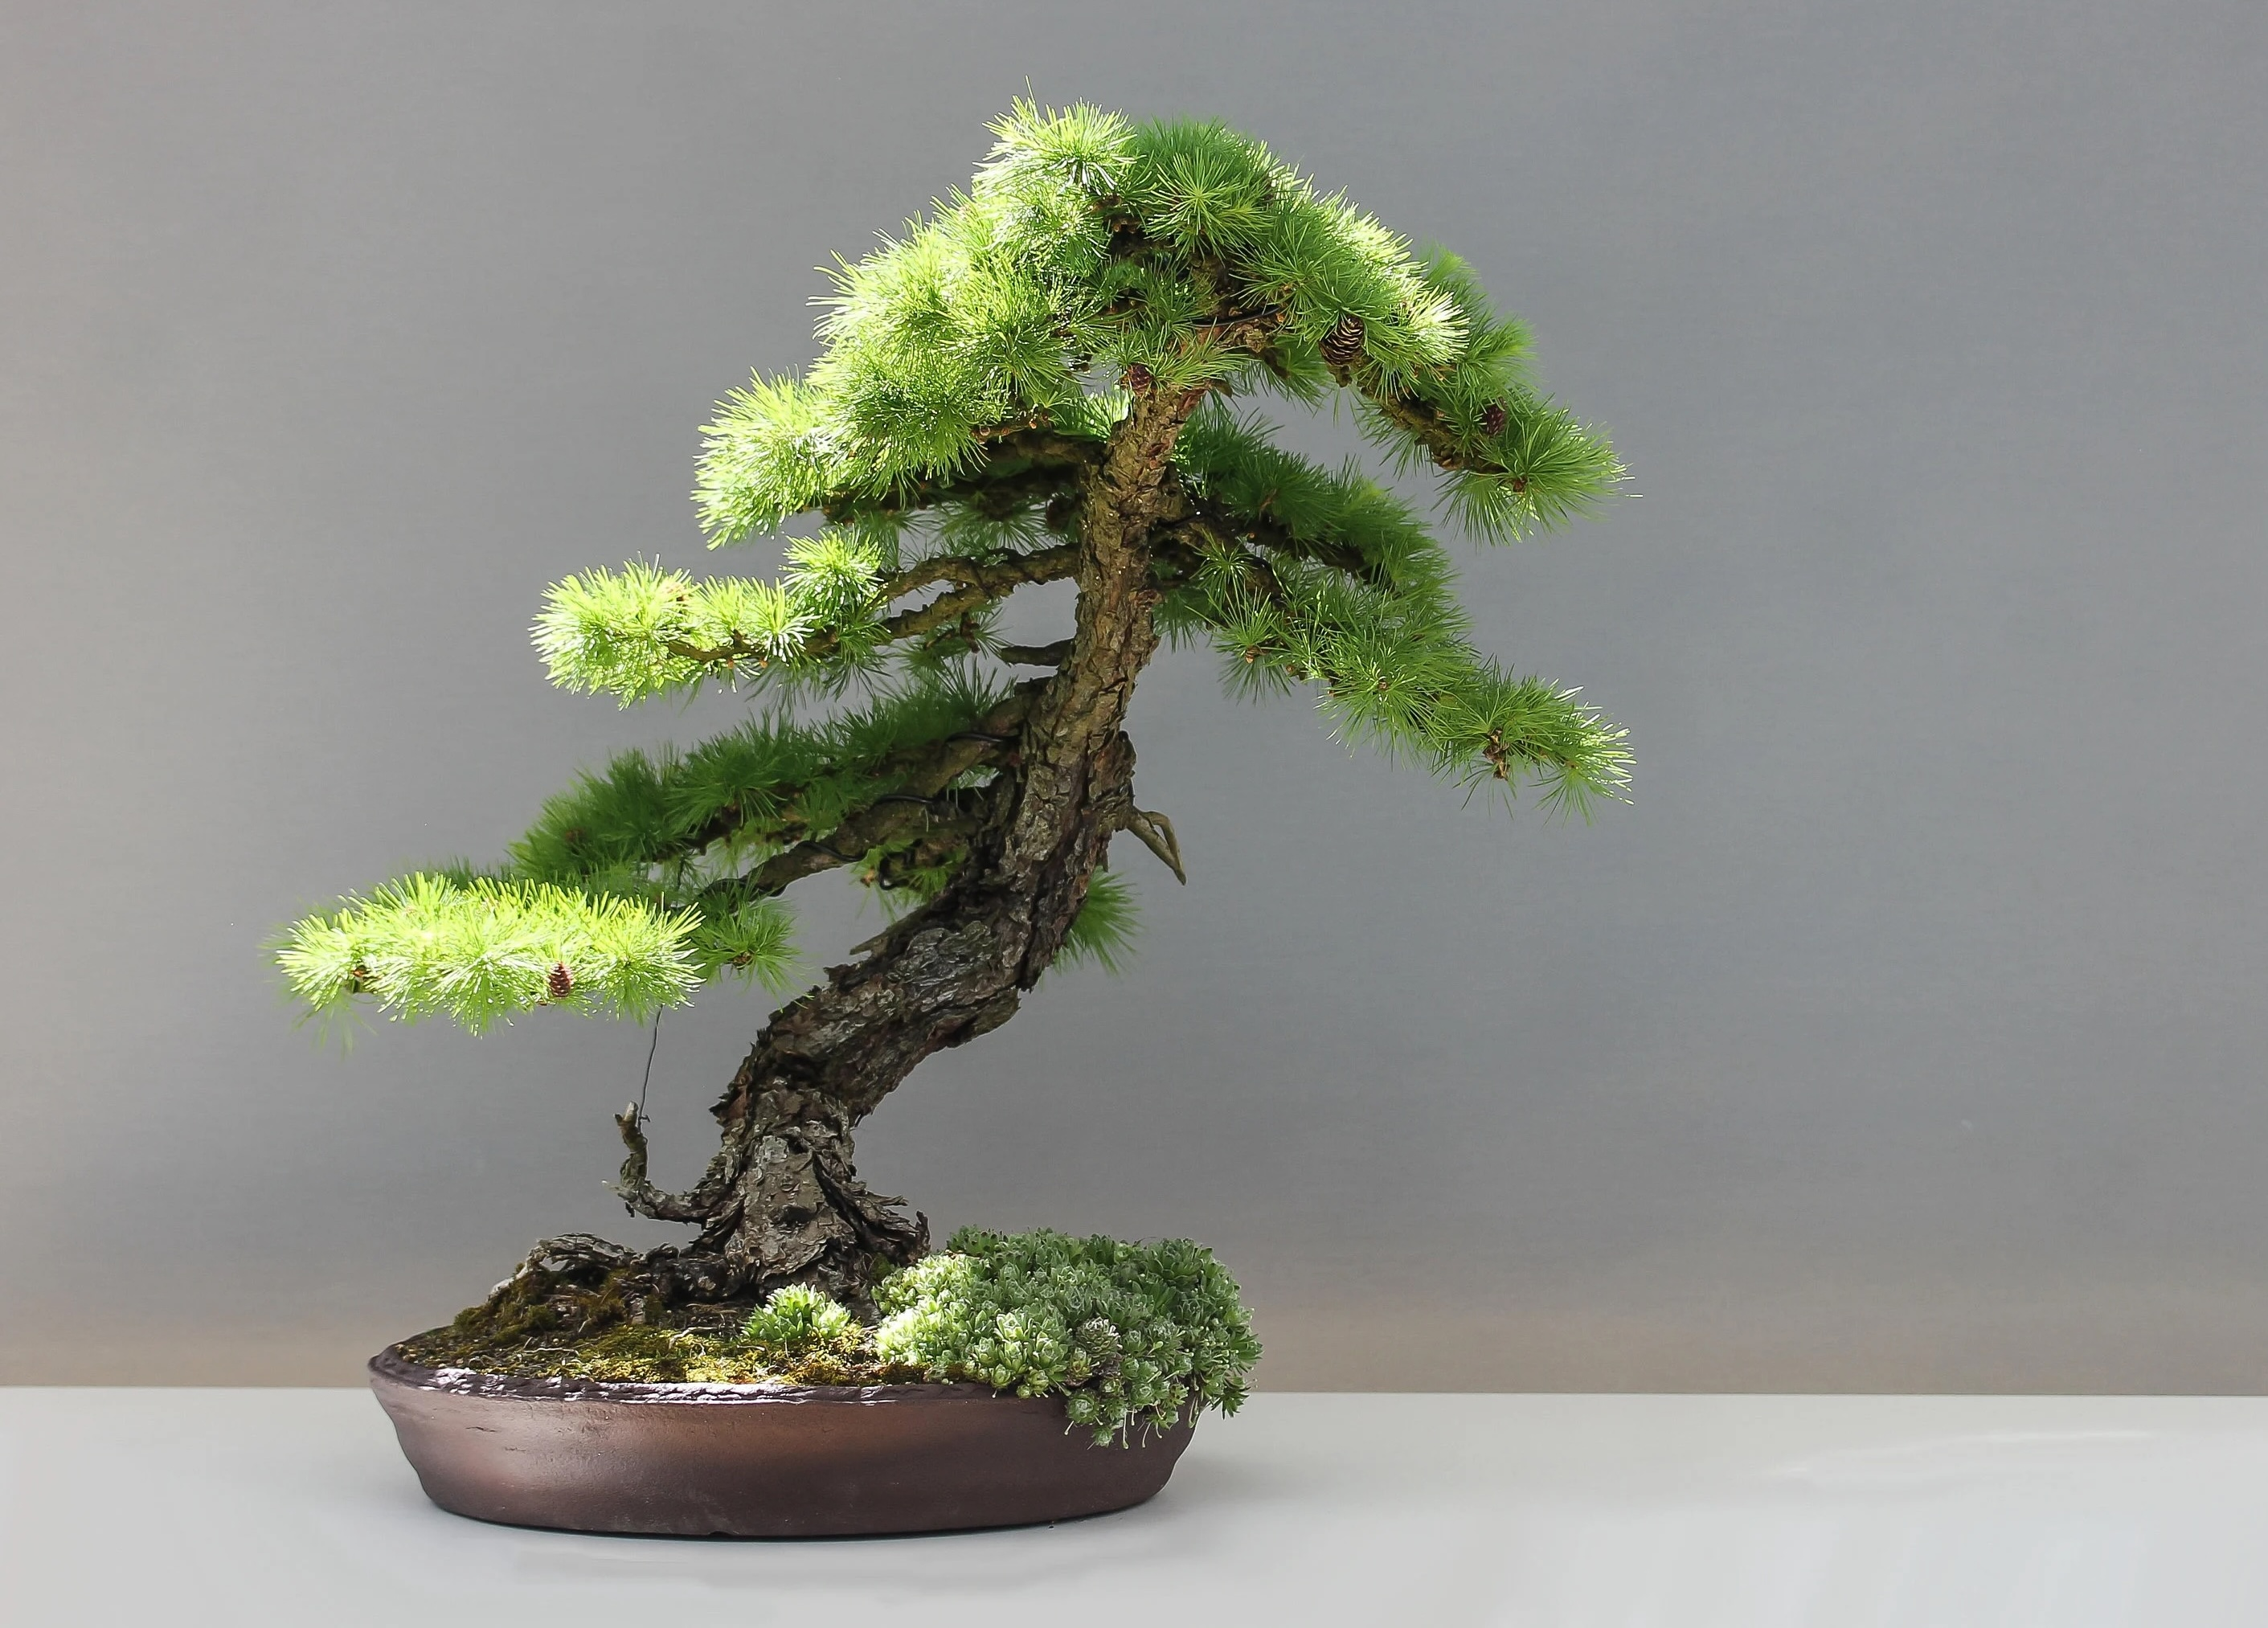
\includegraphics[width=1.0\columnwidth]{2025_11/res/pines_larch.jpg},\centerline{\emph{A Japanese larch (larix kaempferi).}}]
\end{window}

% \smallskip
\topic{\large\sffamily Development of pines in the pre\--bonsai stage}
\label{pre_bonsai}
\noindent
Managing pines in the pre\--bonsai stage differs radically from that of trees in maintenance.
At this stage it is not important to achieve fine ramification or short needles, but rather to build the structure of the plant: thicken the trunk, develop a correct nebari and form healthy branch lines.
Cultivation in wide containers or colanders is ideal, as it promotes the development of fine, vigorous roots.
Fertilisation must be abundant to stimulate growth and develop trunks with natural taper.

Sacrifice branches play a fundamental role. These branches are left to grow freely to thicken specific portions of the trunk and are removed only when their purpose has been fulfilled.
In pre\--bonsai, advanced techniques such as mekiri or tight pinching are not used, as they would limit vigour.
Even needle removal should be avoided: every needle is a source of energy, and reducing them would slow the development of material still in formation.
Trunk shaping is better carried out in autumn and winter, when sap is low, allowing broader, more natural movements without much risk of breakage.

\medskip
\topic{Conclusion}
\noindent
Cultivating a pine bonsai means working in harmony with a precise annual cycle, knowing the specific characteristics of the species you are caring for and respecting the timings and limits imposed by the plant's physiology.
The pine is a slow and rigorous master: it teaches patience, observation and anticipation, because what is done today produces its effects only months later.

The information provided in Diego Fortuna's conferences, reorganised and expanded here, represents a valuable technical resource for anyone wishing to gain a deep understanding of pine bonsai cultivation.
Knowing the differences between varieties, mastering traditional techniques and moving with precision through the annual cycle means establishing a continuous dialogue with the plant, respecting its way of growing.

Only through this understanding and mutual respect is it possible to develop aged, harmonious bonsai full of character.
\closearticle
\clearpage
